% مقایسه شهودی سه رژیم: گاف ثابت، بسته شدن 1/n، بسته شدن نمایی
% نرمال شده به n=2 با Delta=0.66 (مثال دوکیوبیتی) برای دو رژیم متغیر
% سبک مشترک نمودارهای سند پایه‌ها (فقط داخل محیط latin فراخوانی شود)
\tikzset{
	qafbox/.style={
		draw=black!55,
		rounded corners=2pt,
		align=center,
		inner sep=3pt,
		thick,
		fill=white,
		font=\footnotesize\linespread{1}\selectfont,
		minimum height=0.95cm
	},
	qafwide/.style={
		qafbox,
		text width=2.55cm
	},
	qafnarr/.style={
		qafbox,
		text width=2.05cm
	},
	qaftitle/.style={
		font=\small\bfseries\linespread{1}\selectfont,
		align=center
	},
	qafarr/.style={
		-{Latex[length=2.2mm]},
		thick,
		draw=black!65
	},
	qafpanel/.style={
		draw,
		thick,
		rounded corners=4pt,
		inner xsep=8pt,
		inner ysep=8pt
	}
}

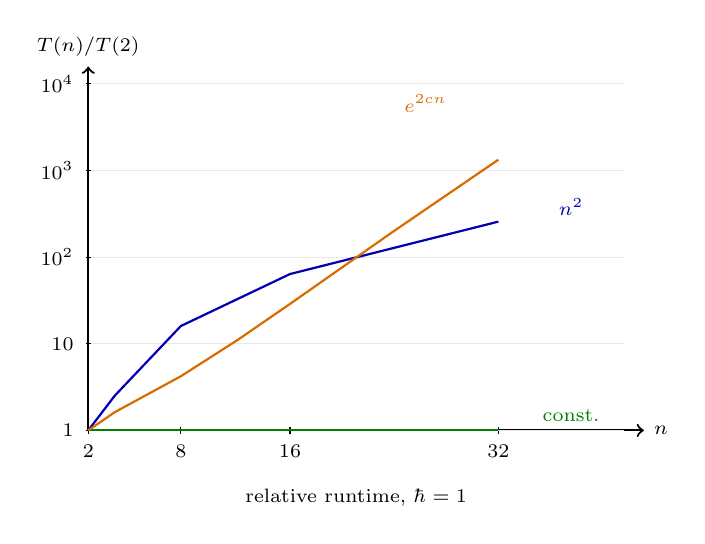
\begin{tikzpicture}[
	x=0.42cm,
	y=0.55cm,
	font=\scriptsize
	]
	% --- left: relative runtime T(n)/T(2) ---
	\draw[->, thick] (0,0) -- (16.8,0) node[right] {$n$};
	\draw[->, thick] (0,0) -- (0,8.4) node[above] {$T(n)/T(2)$};
	\foreach \x/\lab in {0/2, 2.8/8, 6.1/16, 12.4/32} {
		\draw (\x,0.08) -- (\x,-0.08);
		\node[below] at (\x,-0.12) {$\lab$};
	}
	\foreach \y/\lab in {0/1, 2/10, 4/10^{2}, 6/10^{3}, 8/10^{4}} {
		\draw[gray!18] (0,\y) -- (16.2,\y);
		\draw (-0.08,\y) -- (0.08,\y);
		\node[left] at (-0.15,\y) {$\lab$};
	}

	% Independent: T/T2 = 1  (log10 = 0)
	\draw[thick, green!50!black]
		(0,0) -- (12.4,0);
	\node[green!50!black] at (14.6,0.35) {const.};

	% Polynomial alpha=1: T/T2 = (n/2)^2
	% n=2,8,16,32 -> 1, 16, 64, 256
	% y = 2*log10(Trel) so 1->0, 16->2.4, 64->3.61, 256->4.82
	\draw[thick, blue!70!black]
		plot coordinates {
			(0.00,0.00)
			(0.80,0.80)
			(2.80,2.41)
			(6.10,3.61)
			(12.40,4.82)
		};
	\node[blue!70!black] at (14.6,5.15) {$n^{2}$};

	% Exponential c=0.12: T/T2 = exp(0.24(n-2))
	% n=2,8,16,24,32 -> 1, 4.22, 28.8, 196, 1339
	% y=2 log10: 0, 1.25, 2.92, 4.58, 6.25
	\draw[thick, orange!85!black]
		plot coordinates {
			(0.00,0.00)
			(0.80,0.42)
			(2.80,1.25)
			(4.50,2.08)
			(6.10,2.92)
			(9.20,4.58)
			(12.40,6.25)
		};
	\node[orange!85!black] at (10.2,7.55) {$e^{2cn}$};

	\node at (8.1,-1.55) {relative runtime, $\hbar=1$};
\end{tikzpicture}
